\usepackage{booktabs} % improving tables
\usepackage{float}
\usepackage[margin = 1.2in]{geometry} % change the page margins
\usepackage{graphicx} % to use \includegraphics
\usepackage{hyperref} % adding urls using \url
\usepackage[utf8]{inputenc} % makes sure other characters than ASCII can be used
\usepackage{parskip} % makes sure that a line is skipped after every paragraph
\usepackage{subcaption} % for caption of subfigures
\usepackage{tikz} % for graphics, also build front cover using tikz
\usepackage{titlesec, color}
\usepackage{todonotes} % placing todo notes and summarizing them at start of document
\usepackage{wrapfig}

%% Bibliography style
\bibliographystyle{tudelft-report}

%% Change font to sans-serif
\renewcommand{\familydefault}{\sfdefault}

%% Folder with figures
\graphicspath {{figure/}}

%% Acronym
\usepackage{acronym} 

%% Text lay-out
% Customize chapter style
\titleformat
{\chapter} % command
[hang] % shape
{\bfseries \huge} % format
{\thechapter \hspace{5pt} \textcolor{cyan} {$|$} } % label
{0pt}
{\bfseries \Huge } % before-code
[] % after-code

\titlespacing
{\chapter}
{30pt} % Left
{-30pt} % Top
{5pt} % Bottom
%%  Hyperlink colors
\hypersetup{ %setup hyperlinks
    colorlinks,
    citecolor=black,
    filecolor=black,
    linkcolor=black,
    urlcolor=black
}

\setlength{\parindent}{0pt}

%% Tikz settings
\usetikzlibrary{arrows,shapes,positioning,shadows,trees}

%% Front cover, blank page, title page command

\newcommand{\makeCover}{
	%% Create an empty page for cover.
	\clearpage
	\thispagestyle{empty}

 	%% Building cover
	\begin{tikzpicture}[remember picture,overlay]
		\node (picture) at (current page.center)
		{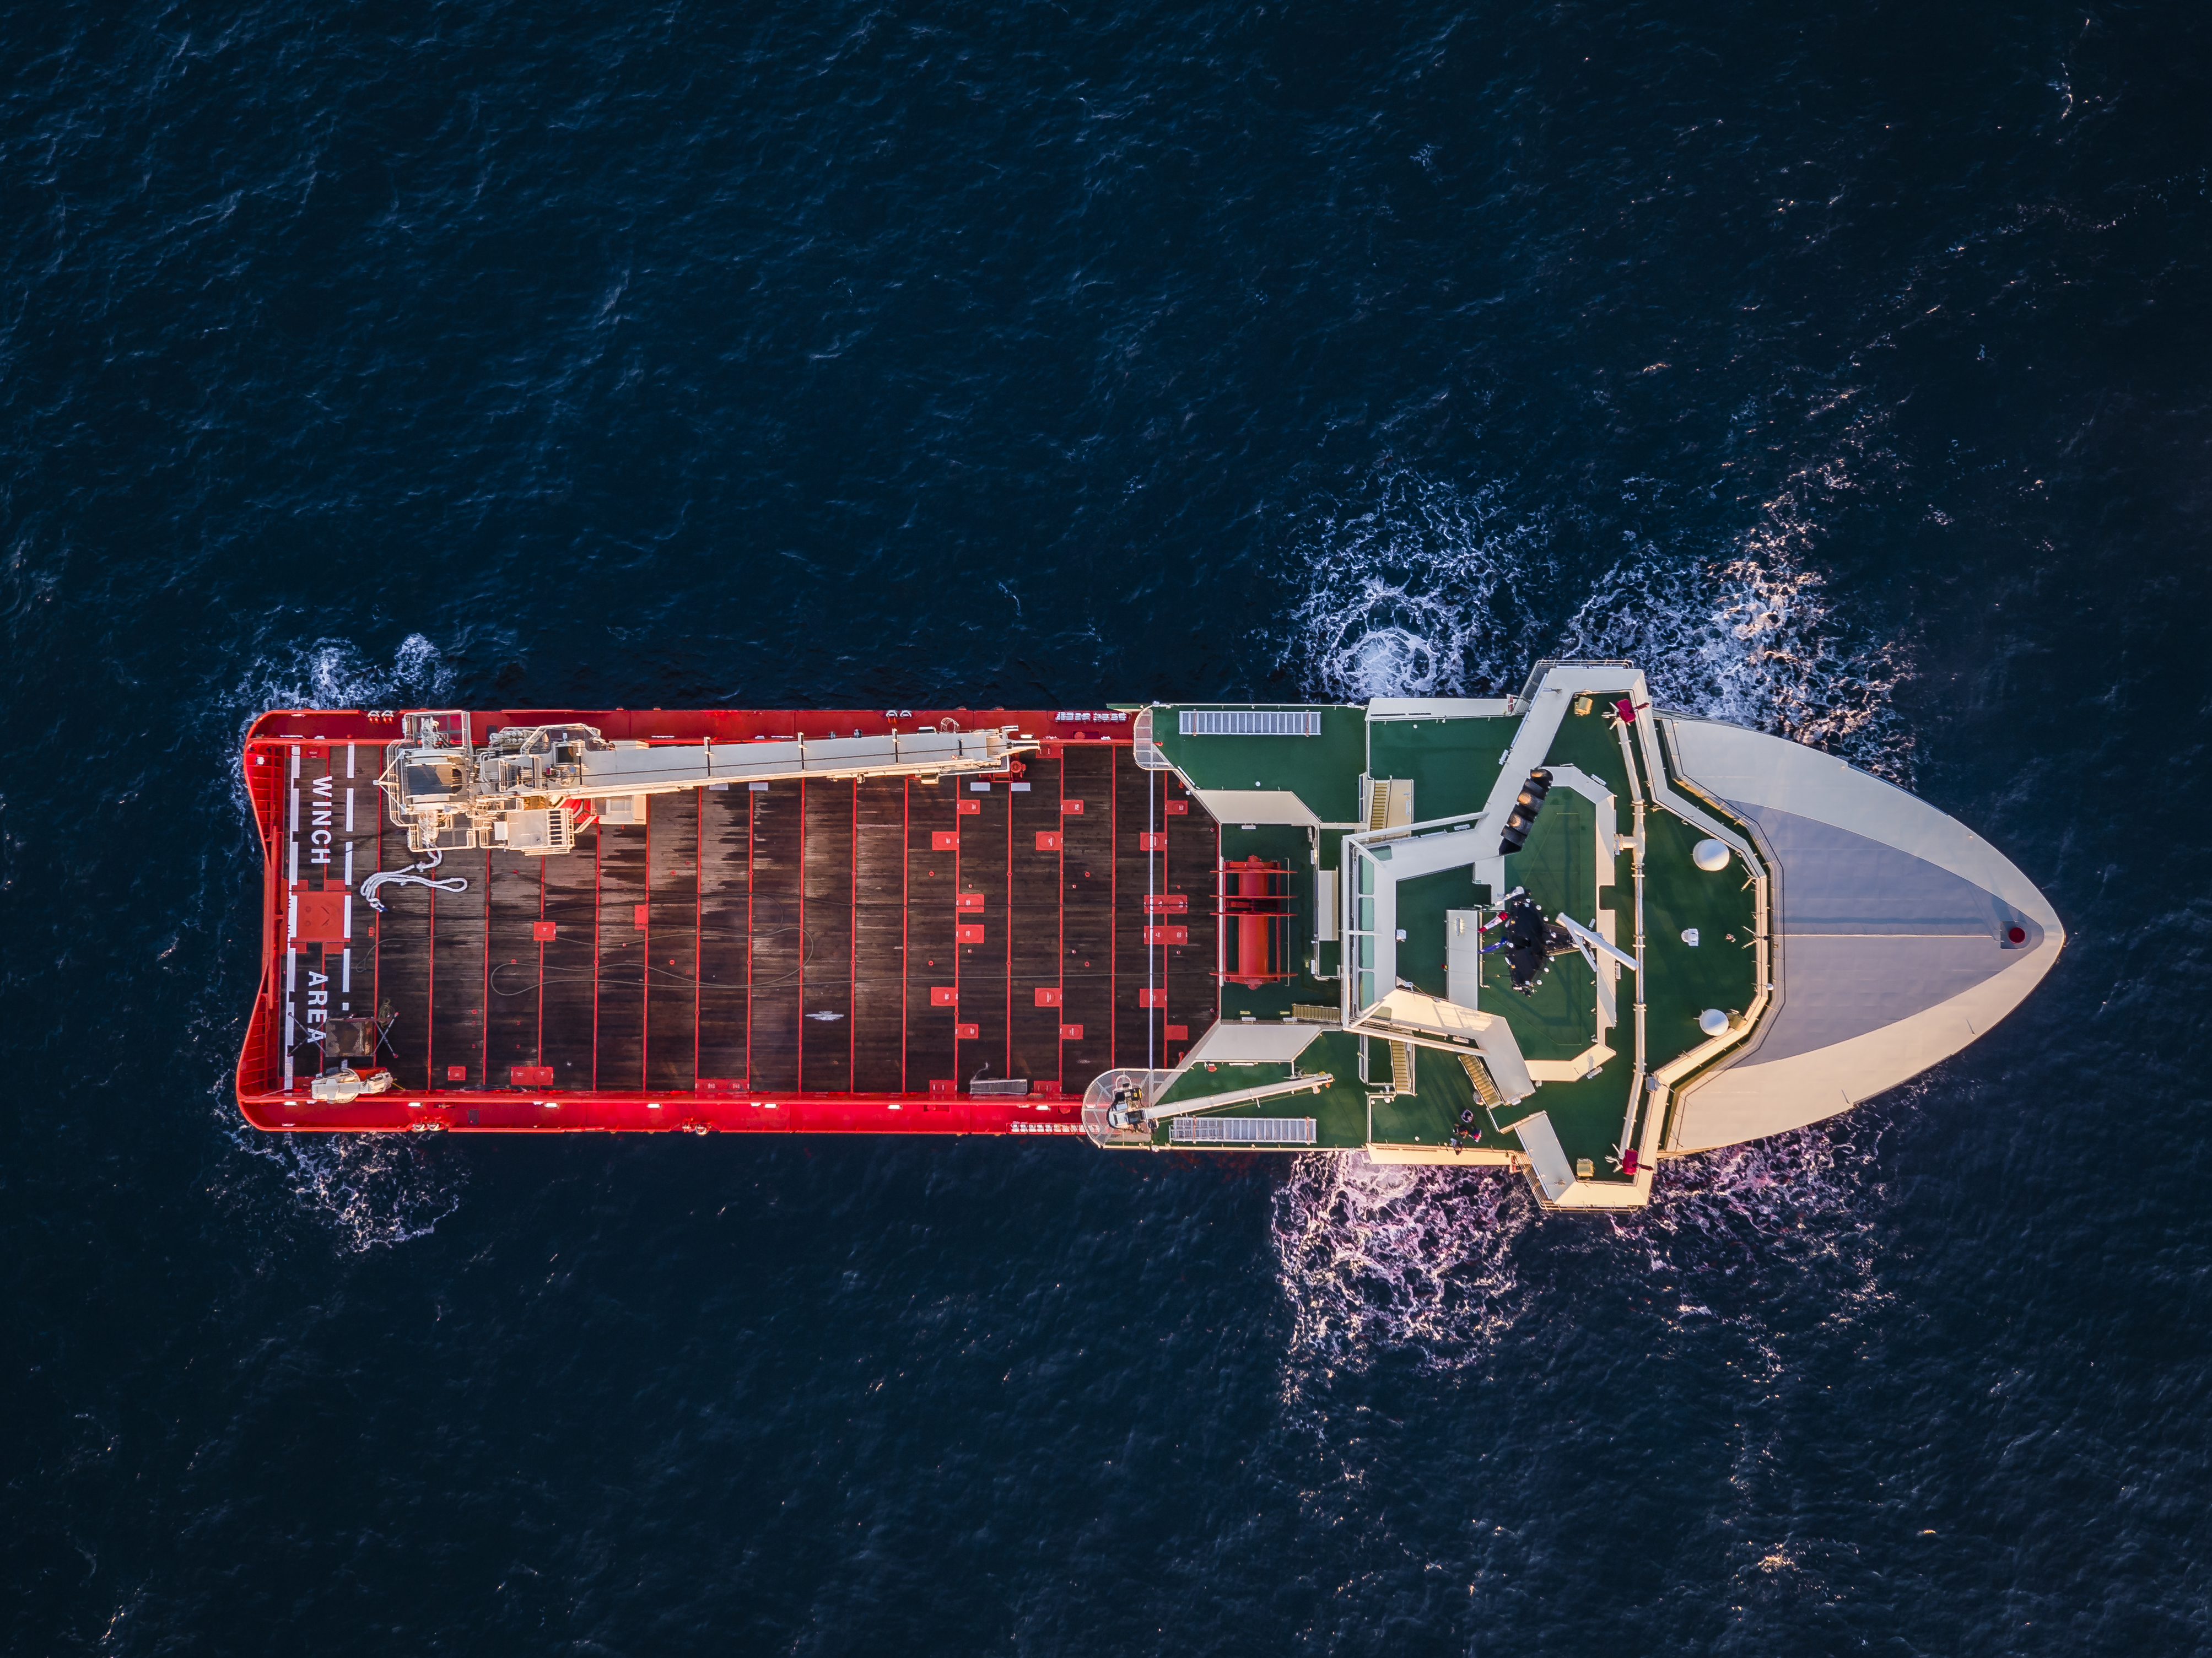
\includegraphics[height=\paperheight, keepaspectratio]{cover_PSV_5000_top.jpg}};
		
		\node (white-glow) at (current page.center) [fill = white, minimum width = \paperwidth, minimum height = \paperheight, opacity = 0.15]{};
		
		\node (title-box-bg) at (current page.east) [fill = gray, minimum width=.5\paperwidth, minimum height=7cm, fill opacity = 0.85, xshift=-.25\paperwidth, yshift=-5cm, text=white] {};
		
		\node (title-box) at (current page.east) [minimum width=.5\paperwidth, minimum height=7cm, align=left, xshift=-.25\paperwidth, yshift=-5cm, text=white] {
			\hspace{.7cm} \Large{MSc Thesis}\\ \\
			\Huge{Current knowledge}\\ \\
			\Large{Model to improve situational awareness of crew}\\ \\
			Ingmar Wever (4161041) \\
			\today
			
		};
	
		\node (black-bar) [fill = black, minimum width=.5\paperwidth, minimum height=0.2cm, xshift=-.25\paperwidth, xshift=.25\paperwidth, yshift = -3.4cm, fill opacity = 0.7] at (title-box){};
		
		\node (cyan-bar) [fill = cyan, minimum width=.5\paperwidth, minimum height=0.2cm, xshift=-.25\paperwidth, xshift=.25\paperwidth, yshift = -3.6cm, fill opacity = 0.7] at (title-box){};
		
		\node (white-bar) [fill = white, minimum width=.5\paperwidth, minimum height=1.5cm, xshift=-.25\paperwidth, xshift=.25\paperwidth, yshift = -4.5cm, fill opacity = 0.95] at (title-box){
		
			\includegraphics[height=1.3cm, keepaspectratio]{TU_Delft_logo_RGB.png}
			\hspace{.8cm}
			\includegraphics[height=.8cm, keepaspectratio]{Damen_logo.png}
		};
	
		
	\end{tikzpicture}
	
	%% Create empty page for two-sided printing
	\clearpage
	\thispagestyle{empty}
	\vspace*{6cm}
	\begin{center}
		This page is intentionally left blank.
	\end{center}

	%% Title page
	\begin{titlepage}
		\newpage
		\setcounter{page}{0}
		
		\centering
		\Large
		\vspace*{3cm}
		\doctitle\\
		\large
		\vspace{1cm}
		\today
		
		\vspace{7cm}
		\normalsize
		\begin{tabular}{lll}
			Student: & Ingmar Wever & 4161041 \\
			Project duration: & \multicolumn{2}{l}{September 2017 -- July 2018} \\
			& & \\
			Supervisors: & Dr.\ ir.\ Robert Hekkenberg & TU Delft, Maritime Technology \\
			& Prof.\ Dr. \ Mark Neerincx & TU Delft, Computer Science \\
			& Toine Cleophas & Damen Shipyards
		\end{tabular}

\end{titlepage}
		
}
	